\subsection{Stream Partitioning}
We use the Geohash~algorithm~\cite{geohash} to balance load and partition incoming data streams across processing resources. Geohash divides the earth into a hierarchy of bounding boxes identified by Base 32 strings; the longer the Geohash string, the more precise the bounding box. Figure~\ref{fig:geohash} illustrates this hierarchy. Most of the eastern United States is contained within the bounding box described by Geohash string \emph{D}, while \emph{DJ} encompasses substantial parts of Florida, Georgia, and Alabama. The bounding box \emph{DJKJ} (highlighted in red) contains Tallahassee, Florida. This hierarchical representation enables \textsc{Rivulet} to cope with both low- and high-density regions: several resources may be tasked with managing streams originating in and around large cities, while rural areas fall under the purview of a single node.

\begin{figure}
    \centerline{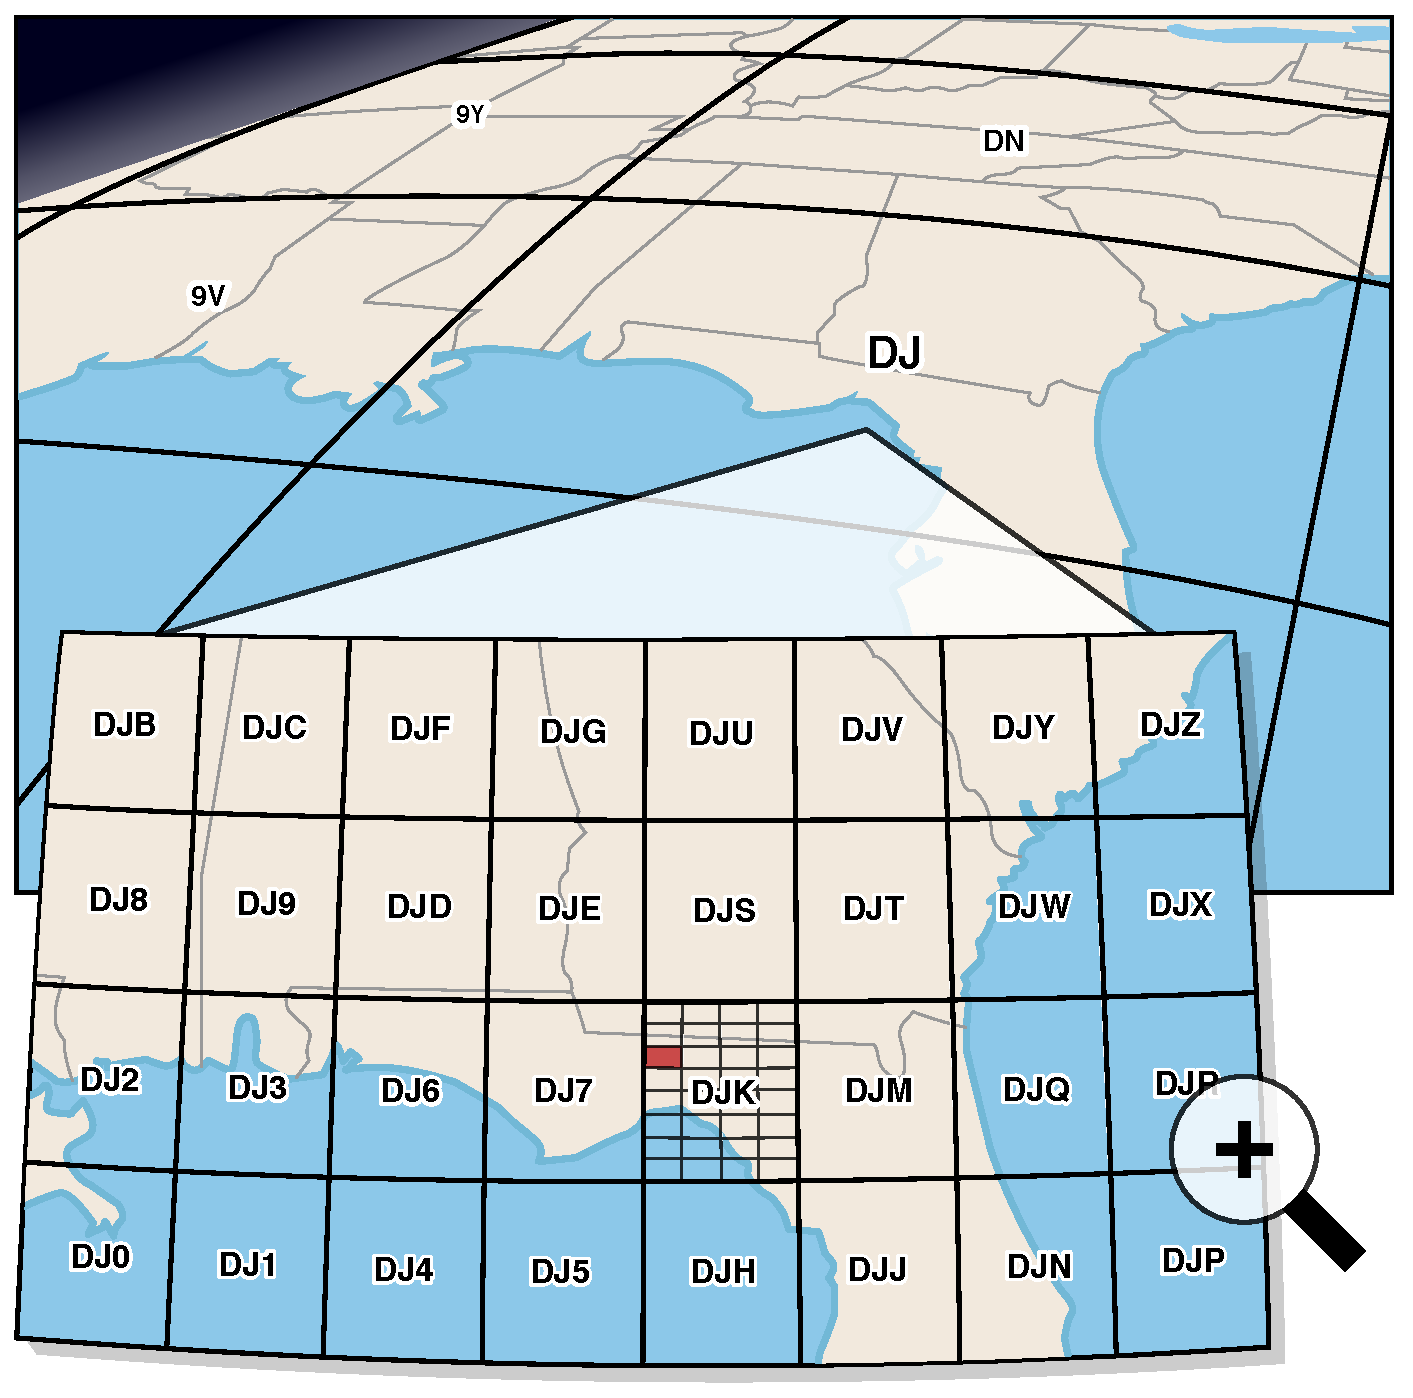
\includegraphics[width=3.5in]{figures/geohash.pdf}}
    \caption{A demonstration of the Geohash algorithm. Each additional character in a Geohash string describes a finer-grained region; Geohash \emph{DJ} contains substantial parts of Florida, Georgia, and Alabama, USA, while \emph{DJKJ} (highlighted in red) encompasses Tallahassee, the capital of Florida.}
    \label{fig:geohash}
\end{figure}

To achieve fine-grained control over our Geohash partitions, we operate at the bit level rather than Base 32 character level when routing streams. Each bit added to a Geohash string reduces its scope by half, with each character represented by five bits ($2^5 = 32$). In other words, a four-character Geohash string represents 20 spatial subdivisions. This property allows us to manage and allocate resources across a wide variety of observational densities.

\begin{figure}
    \centerline{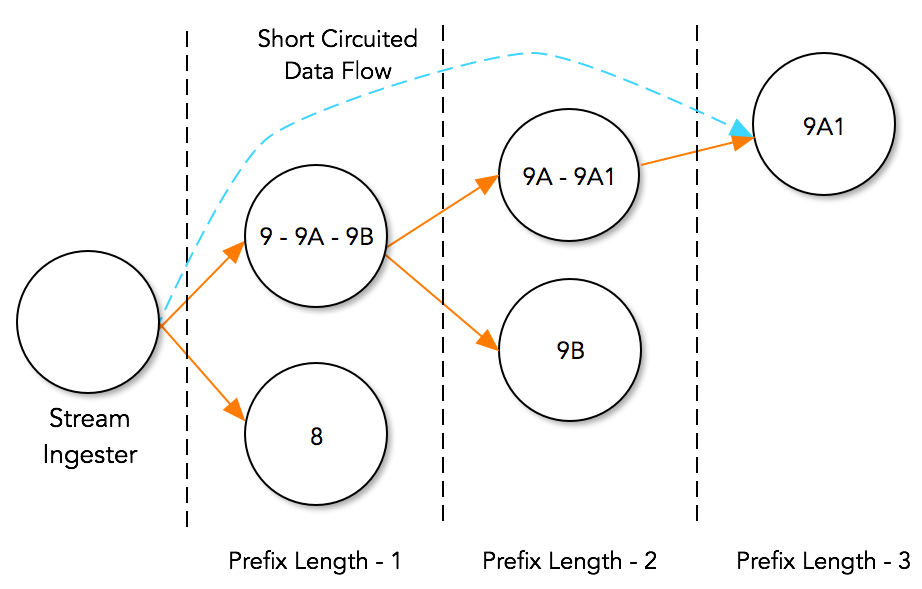
\includegraphics[width=3.5in]{figures/stream-partitioning.png}}
    \caption{An example of the stream partitioning based on Geohashes of the stream packets}
    \label{fig:stream-partitioning}
\end{figure}
